\documentclass[12pt]{beamer}
\usepackage{mathtools}
\usepackage{makecell}
\usepackage{caption}
\usepackage{ragged2e}
\usepackage{paralist}
\usepackage{tcolorbox}
\captionsetup[figure]{labelformat=empty}
\useoutertheme{infolines}
\usetheme{default}
\usefonttheme{serif}
%\usefonttheme{structuresmallcapsserif}
\hypersetup{colorlinks=true,linkcolor=blue}
\setbeamertemplate{navigation symbols}{}
\setbeamertemplate{footline}[frame number]{}
%\setbeamertemplate{footline}{}
\author{Mittereder, \textit{et. al.}}
\definecolor{darkgreen}{rgb}{0,.5,0}
\setlength{\parskip}{.1in}
\newcommand{\freakingtilde}{\raisebox{0.5ex}{\texttildelow}}
\begin{document}

%----------------------------------------------------------------------------
\begin{frame}[c]{}

\begin{center}
\Large

Improving Political Discussion on Social Media
with Automated Bot Intervention

\footnotesize
\textbf{Garrett McKenzie, Bethanie Hackett, Laura Rider}\\
\smallskip
\scriptsize
Faculty advisor: Stephen Davies \\
\medskip
Dept of Computer Science\\
University of Mary Washington\\
Fredericksburg, Virginia, USA\\
\bigskip
\bigskip
\scriptsize
Sixth Annual Network for Undergraduate Research in Virginia (NURVa 2025)\\
\bigskip
\scriptsize
Nov.~1, 2025\\
\texttt{https://github.com/divilian/frozone}
\end{center}

\end{frame}

%----------------------------------------------------------------------------
\begin{frame}[c]{Politically polarized online conversation}
% GM
\small
\begin{center}
Many scholars have observed a degradation in political conversation.
\end{center}

\begin{columns}[c,onlytextwidth]
  \begin{column}{0.2\textwidth}
    \centering
    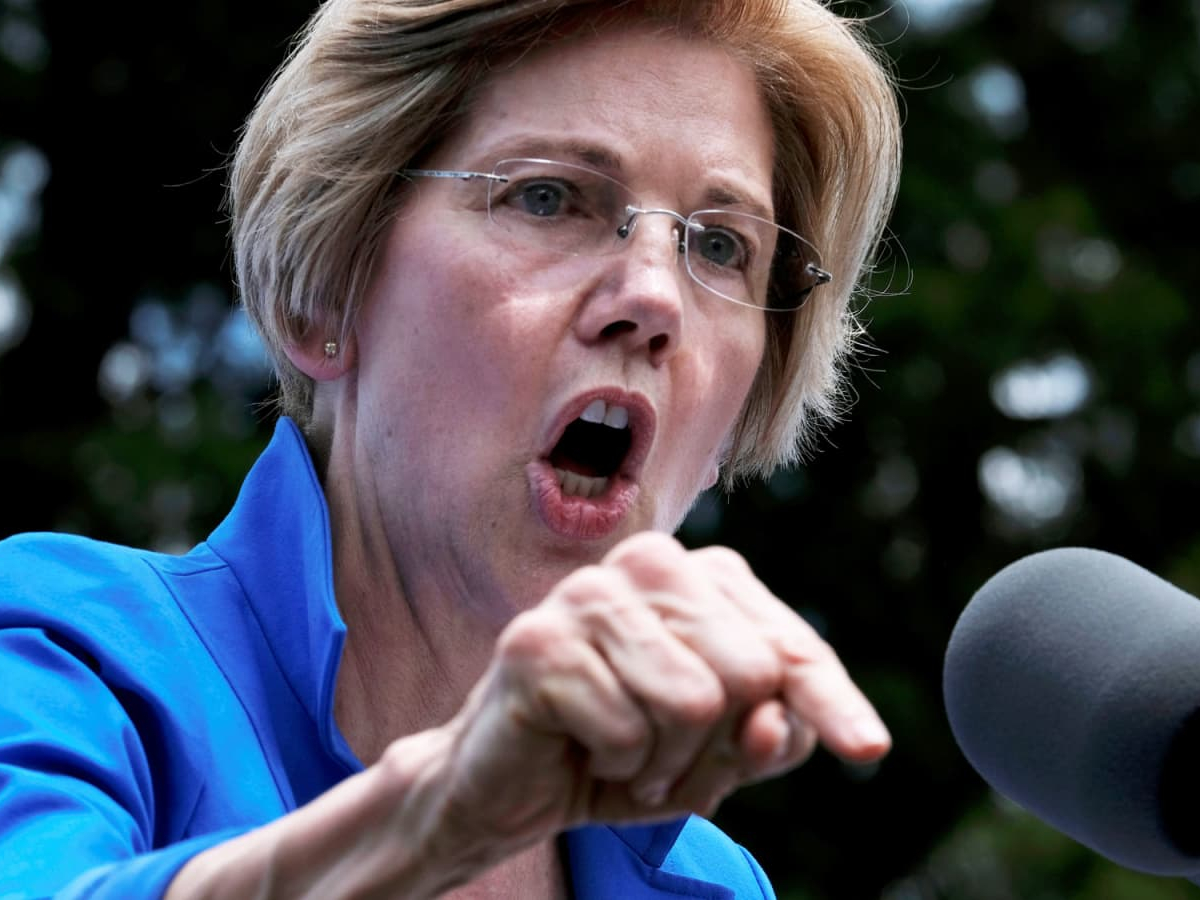
\includegraphics[width=\linewidth]{warren.jpg}\\
    \bigskip
    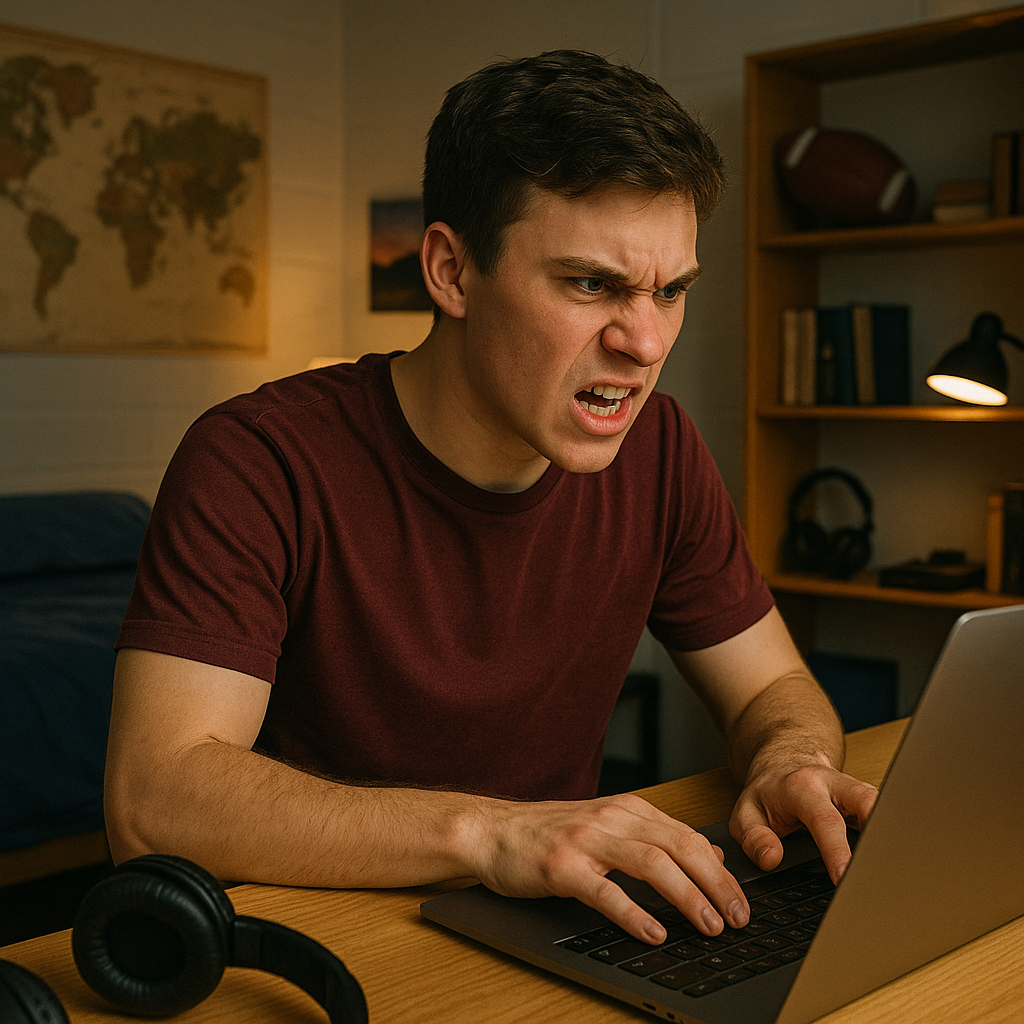
\includegraphics[width=\linewidth]{angryGuy.png}
  \end{column}

  \begin{column}{0.01\textwidth}\hfill\end{column}
  \begin{column}{0.5\textwidth}
  This includes a rise in:\\
    \RaggedRight
    \begin{compactitem}
        \item misinformation/disinformation
        \item political intolerance
        \item erroneous reasoning
        \item affective polarization
        \item toxic speech
        \item echo chambers
        \item biased viewpoints
    \end{compactitem}
  \end{column}

  \begin{column}{0.2\textwidth}
    \centering
    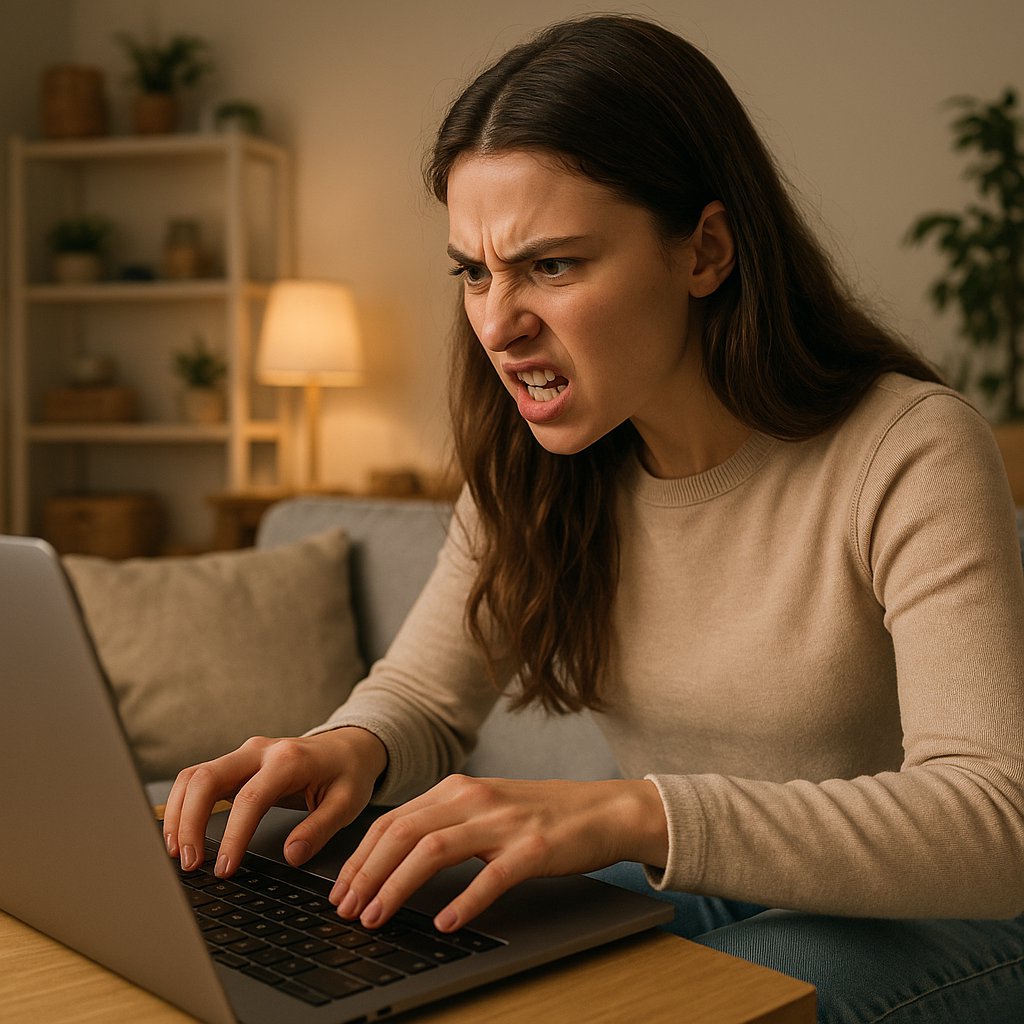
\includegraphics[width=\linewidth]{angryGirl.png} \\
    \bigskip
    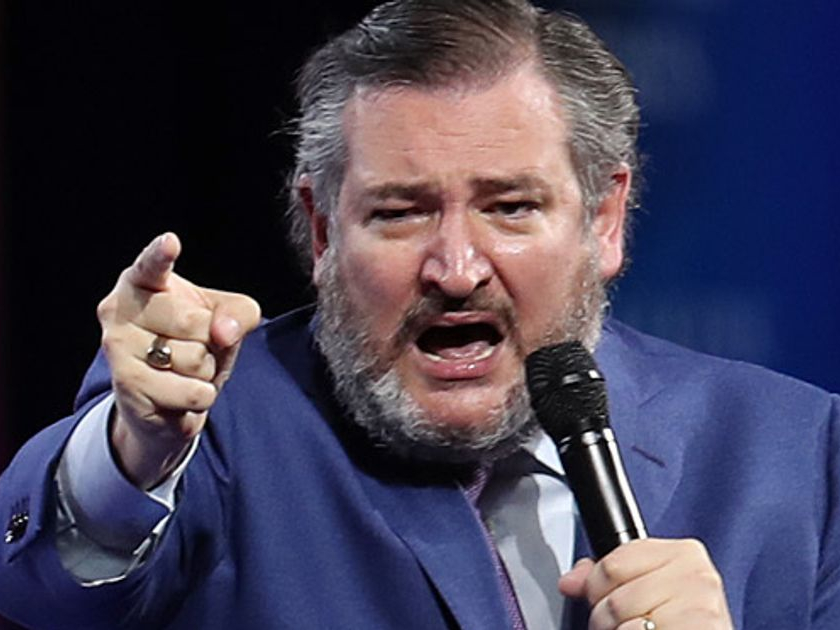
\includegraphics[width=\linewidth]{cruz.jpg}
  \end{column}
\end{columns}

\vspace{-.1in}
\begin{center}
This erosion of trust and communication is alarming for a democracy.\\
\pause
\large Is there a way to improve it?
\end{center}

\end{frame}
%----------------------------------------------------------------------------
\begin{frame}[c]{Main idea}
% BH

Train a Large Language Model (LLM) to imitate a human social media participant.

\vspace{-.3in}
\pause

\makebox[\textwidth][c]{%
  \begin{columns}[c,totalwidth=0.7\textwidth]
    \begin{column}{0.3\textwidth}
    \begin{center}
    \LARGE ``FroBot''
    \end{center}
    \end{column}
    \begin{column}{0.7\textwidth}
    
\includegraphics[width=0.4\textwidth]{frozone.png}
    \end{column}
\end{columns}
}

\pause
    
The FroBot will observe and intervene in online conversations:

\small
\begin{compactitem}
\item reduce affective ``temperature''
\item non-threateningly call out misinformation
\item gently identify sources of bias
\item respectfully correct fallacies of reasoning
\end{compactitem}

\end{frame}
%--------------------------------------------
\begin{frame}[c]{Using LLMs as ``personas''}
% GM

\scriptsize
\begin{itemize}
\itemsep2em
\item Deshpande, A., Murahari, V., Rajpurohit, T., Kalyan, A., \& Narasimhan, K. (2023). \textbf{Toxicity in chatgpt: Analyzing persona-assigned language models.} In H. Bouamor, J. Pino, \& K. Bali (Eds.), \textit{Findings of the Association for Computational Linguistics: EMNLP 2023} (pp.~1236–1270).

\item Ferraro, A., Galli, A., Gatta, V. L., Postiglione, M., Orlando, G. M., Russo, D., Riccio, G., Romano, A., \& Moscato, V. (2024). \textbf{Agent-Based Modelling Meets Generative AI in Social Network Simulations.} arXiv preprint arXiv:2411.16031.

\item Törnberg, P., Valeeva, D., Uitermark, J., \& Bail, C. (2023). \textbf{Simulating Social Media Using Large Language Models to Evaluate Alternative News Feed Algorithms.} arXiv preprint arXiv:2310.05984.
\end{itemize}


\end{frame}
%----------------------------------------------------------------------------
\begin{frame}[c]{Improving online political conversation}
% BH

\scriptsize
\begin{itemize}
\itemsep1em

\item Argyle, L. P., Busby, E., Gubler, J., Bail, C., Howe, T., Rytting, C., \& Wingate, D. (2023). \textbf{AI Chat Assistants can Improve Conversations about Divisive Topics.} arXiv preprint arXiv:2302.07268.

\item Bonaldi, H., Chung, Y.-L., Abercrombie, G., \& Guerini, M. (2024). \textbf{NLP for Counterspeech against Hate: A Survey and How-To Guide.} In K. Duh, H. Gomez, \& S. Bethard (Eds.), \textit{Findings of the Association for Computational Linguistics: NAACL 2024} (pp. 3480–3499).

\item Saha, P., Agrawal, A., Jana, A., Biemann, C., \& Mukherjee, A. (2024). \textbf{On Zero-Shot Counterspeech Generation by LLMs.} arXiv preprint arXiv:2403.14938.

\item Tessler, M. H., Bakker, M. A., Jarrett, D., Sheahan, H., Chadwick, M. J., Koster, R., Evans, G., Campbell-Gillingham, L., Collins, T., Parkes, D. C., Botvinick, M., \& Summerfield, C. (2024). \textbf{AI can help humans find common ground in democratic deliberation.} \textit{Science}, 386(6719).
\end{itemize}

\end{frame}
%----------------------------------------------------------------------------
\begin{frame}[c]{Experiment: purpose and methodology}
% LR

Purpose: determine whether and how the FroBot approach can increase quality of a political dialogue.

\pause
Recruit volunteer participants to engage in online political dialogue (30 mins). 
\pause

Each participant will and be put in a chat room with:

\begin{enumerate}
\itemsep.1em
\item One ``CoolBot'': mimics a generic social media user
\item One ``HotBot'': aims to spark disagreement and controversy
\item One FroBot: aims to improve dialogue quality
\end{enumerate}

\pause
Capture full chat transcripts for later analysis.

\pause
Administer surveys for demographics, political leanings, and social media use.

\end{frame}
%--------------------------------------------
\begin{frame}[c]{Fooling the user}
% LR

\begin{columns}[c,onlytextwidth]
  \begin{column}{0.25\textwidth}
    \centering
    
\includegraphics[width=\linewidth]{surprised1.png}
  \end{column}

  \begin{column}{0.03\textwidth}\hfill\end{column}
  \begin{column}{0.5\textwidth}
An ethical consideration: are we being untruthful ourselves by deploying a 'bot in the guise of a human?
  \end{column}

  \begin{column}{0.03\textwidth}\hfill\end{column}
  \begin{column}{0.2\textwidth}
    \centering
    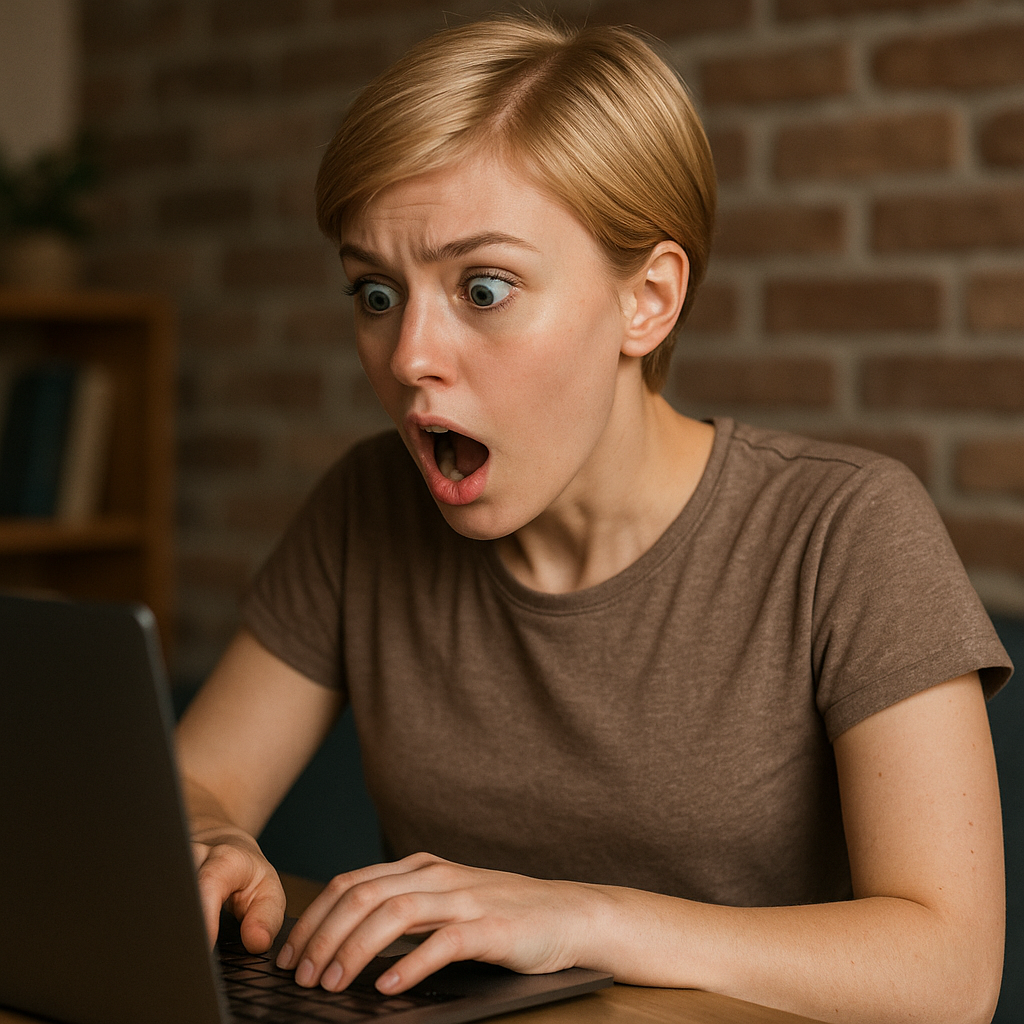
\includegraphics[width=\linewidth]{surprised2.png}
  \end{column}
\end{columns}

\pause

Well.....yes.

\pause

Our project's purpose is to determine \textit{what effect a FroBot might have if deployed.}

Balancing ethical costs vs.~societal benefits is something to consider later. (The question is moot if FroBot doesn't work.)

\end{frame}
%--------------------------------------------
% GM
\begin{frame}[c]{LLM fine-tuning}

To fine-tune a LLM means to take an already-trained model and train it further on a smaller, task-specific dataset so it adapts to a particular style, domain, or objective. 

In this case, we want to fine-tune our LLM to respond effectively to instances of unproductive dialogue, which vanilla models don't always do well out-of-the-box. We provide data like such for training:

\tiny
\ttfamily
\begin{tabbing}
\hspace{1em}\=\hspace{2em}\=\kill % tab stops
\{ \\
\> "systemInstruction": \{ \\
\>\> "role": "system", \\
\>\> "parts": [ \{ "text": "You are skilled in countering toxic behavior." \} ] \\
\> \}, \\
\> "contents": [ \\
\>\> \{ "role": "user",  "parts": [ \{ "text": "A: Hello!" \} ] \}, \\
\>\> \{ "role": "model", "parts": [ \{ "text": "(pass)" \} ] \}, \\
\>\> \{ "role": "user",  "parts": [ \{ "text": "B: A is stinky!" \} ] \}, \\
\>\> \{ "role": "model", "parts": [ \{ "text": "F: No need to get personal, A smells great." \} ] \}, \\
\> ] \\
\}
\end{tabbing}

\end{frame}
%--------------------------------------------
\begin{frame}[c]{Architecture}
% GM
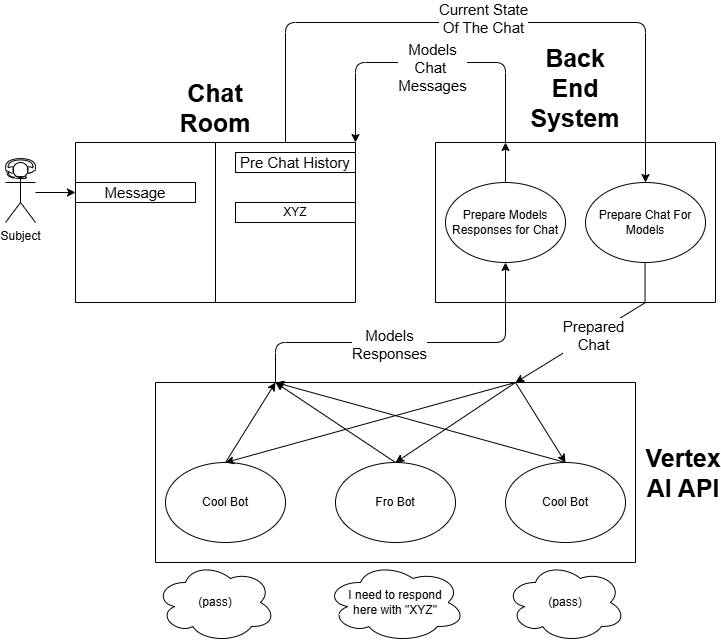
\includegraphics{Experiment Design.drawio.png}
\end{frame}
%--------------------------------------------
\begin{frame}[c]{LLM prompts}
% LR

What role is the LLM playing?
\begin{tcolorbox}[colback=black,colframe=red!75!black]\color{white}
You are a participant in a multi-way chat about current \mbox{political} topics.
\end{tcolorbox}
\pause
What tasks should the LLM perform?
\begin{tcolorbox}[colback=black,colframe=blue!75!black]\color{white}
Decide whether to respond. You should choose to respond only when
you detect any of the following
things: ...\end{tcolorbox}

\end{frame}
\begin{frame}[c]{LLM prompts}

How should the LLM perform tasks?
\begin{tcolorbox}[colback=black,colframe=red!75!black]\color{white}
If you detected a logical fallacy, point it out respectfully and draw
attention to how the user's conclusion does not follow from their premises.
\end{tcolorbox}
\pause
What are specific techniques?
\begin{tcolorbox}[colback=black,colframe=blue!75!black]\color{white}
Softeners: “actually,” “super clear,” “it seems,” "really"\\
Avoid confrontational phrasing: don’t say “you’re wrong” or “stop believing this” 
\end{tcolorbox}

\end{frame}
%--------------------------------------------
\begin{frame}[c]{Demo}
% BH

\textit{BH inserts her demo video of a manually-orchestrated human/FroBot/HotBot interaction.}

\end{frame}
%--------------------------------------------
\begin{frame}[c]{Next steps}
% LR

We're fine-tuning our LLMs on select training data, and refining our prompts.

\pause
Later this month we'll conduct our experiment with student volunteers from UMW's DATA 101 and CPSC 110 courses.
\pause


\begin{columns}[c,onlytextwidth]
  \begin{column}{0.6\textwidth}
After analyzing experimental data, we plan to build an agent-based model (ABM) this spring to test FroBot's effect in a larger social network context.
  \end{column}
  \begin{column}{0.4\textwidth}
    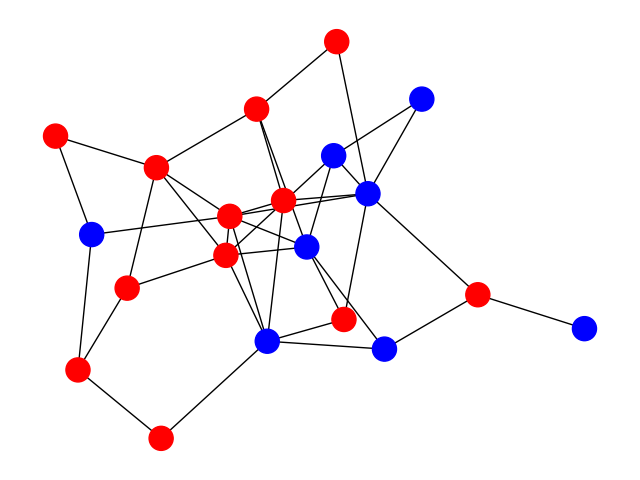
\includegraphics[width=\linewidth]{agraph.png}
  \end{column}
\end{columns}

\end{frame}
%--------------------------------------------
\begin{frame}[c]{}

\begin{center}
\Large

Improving Political Discussion on Social Media
with Automated Bot Intervention

\footnotesize
\textbf{Garrett McKenzie, Bethanie Hackett, Laura Rider}\\
\smallskip
\scriptsize
Faculty advisor: Stephen Davies \\
\medskip
Dept of Computer Science\\
University of Mary Washington\\
Fredericksburg, Virginia, USA\\
\bigskip
\bigskip
\scriptsize
Sixth Annual Network for Undergraduate Research in Virginia (NURVa 2025)\\
\bigskip
\scriptsize
Nov.~1, 2025\\
\texttt{https://github.com/divilian/frozone}
\end{center}

\end{frame}
%----------------------------------------------------------------------------

\end{document}
